\section{Design}
\label{s:gen}

To find integer errors, \sys first compiles the C source code to the
LLVM intermediate representation~(IR).  \sys then examines the IR to
find integer operations, and for each operation, \sys generates a
set of predicates on the program's variables that would have to be
true in order for that integer operation to have an error.  Finally,
\sys feeds the constraints for each integer operation into the
Boolector constraint solver for deciding satisfiability.  If the
solver answers ``satisfiable'' with an assignment of variables,
there is a potential integer error that could be triggered with
that assignment.  This workflow is shown in \autoref{f:flow}.

The central challenge is reducing the complexity of these predicates,
so that the solver can run efficiently.  This section describes how
\sys generates the predicates.

\begin{figure}
\centering
\resizebox{\linewidth}{!}{
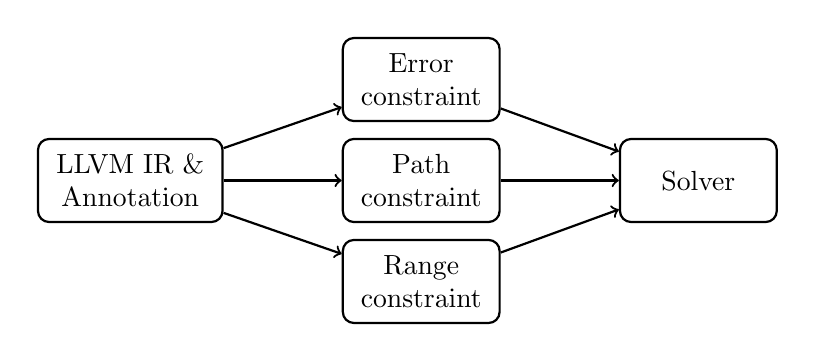
\begin{tikzpicture}[
	block/.style={
		rectangle, rounded corners,
		draw=black, thick,
		text width=5em, minimum height=3em, text centered
	},
	line/.style={draw, thick, ->},
	]
	\matrix[row sep=2mm, column sep=15mm] {
		& \node [block] (ec) {Error constraint}; & \\
		\node [block, text width=6em] (ir) {LLVM IR \& Annotation};
		& \node [block] (pc) {Path constraint};
		& \node [block] (sol) {Solver}; \\
		& \node [block] (rc) {Range constraint}; & \\
	};

	\path [line] (ir) -- (ec);
	\path [line] (ir) -- (pc);
	\path [line] (ir) -- (rc);
	\path [line] (ec) -- (sol);
	\path [line] (pc) -- (sol);
	\path [line] (rc) -- (sol);
\end{tikzpicture}

}
\caption{\sys's workflow.  It generates predicates from the LLVM
intermediate representation~(IR) and user annotations, and then feeds
the predicates to a solver for satisfiability testing.}
\label{f:flow}
\end{figure}

\subsection{Out-of-Bounds Predicate Generation}
\label{s:gen:oob}

%From the definition in \autoref{s:sema:sec},
To find integer errors, \sys needs to detect integer operations
that violate the corresponding in-bounds requirements.
To do so, for each integer operation \sys derives
the negation of its in-bounds requirement, namely out-of-bounds~(OOB) predicate,
satisfying which implies an error.

\paragraph{Arithmetic operations.}
Take multiplication for an example.  Given two $n$-bit unsigned
integers $x$ and $y$, the in-bounds requirement is that their product
cannot overflow $\uintmax(n)$.  There are several possible OOB
predicates \sys could generate.
A \naive form is:
\begin{equation*}
x \neq 0 \land \uintmax(n) /_u x > y.
\end{equation*}
Another possible predicate is to use a $2n$-bit
multiplier~\cite{molnar:catchconv}: extend $x$ and $y$ to $2n$ bits
and flag an error if any of the most significant $n$ bits of the
product is 1.  This is conceptually equivalent to:
\begin{equation*}
x_{2n} \times y_{2n} > \uintmax(n).
\end{equation*}
Both forms would hurt the solver's performance noticeably
(see \autoref{s:eval:perf} for a performance comparison).
%
\sys reuses a specialized multiplication overflow detection predicate
from the Boolector constraint
solver~\cite[\chapterautorefname~3.5]{brummayer:phd}, which can be
solved far more efficiently without computing the product.  The
detailed implementation of the predicate is beyond the scope of
this paper.

\paragraph{Shift.}
The OOB predicate \sys generates for a $n$-bit shift operation
$x \shl y$ or $x \shr y$ is a simple comparison $y \geq n$, where
$y$ is the number of bits to shift.

\paragraph{Conversion.}
As defined \autoref{s:sema:sec}, \sys deals with conversions
in the following cases.

To detect tautological comparisons, \sys derives a predicate from
each comparison.  If the predicate is trivially true or false,
and it resulted from an integer conversion within that function, \sys
reports the conversion as an integer error.

For an array index $x$, \sys generates an OOB predicate $x <_s 0$.
\sys implements a front-end plugin to recognize array indices.

Similarly, for a data size $x$, \sys generates an OOB predicate $x <_s 0$.
\sys requires user-provided annotations on ``size'' function parameters.  As for
the Linux kernel, we annotate the ``size'' parameters in functions like \cc{memcpy},
\cc{copy_from_user}, and \cc{sock_alloc_send_skb}.

\subsection{Path Predicate Generation}
\label{s:gen:path}

\sys generates a path predicate for each integer operation, that encodes
the constraints on the variables that arise from preceding operations
in the function's control flow.  These constraints arise from two general
sources: assignments to variables by preceding operations, and conditional
branches along the execution path.  Satisfying the path predicate with
a given set of variable assignments means that the integer operation is
reachable from the start of its function with those variable values.
The path predicate is used to filter out integer errors that cannot
happen due to previous statements in a function, such as assignments or
explicit overflow checks.

Let's consider loop-free programs first.
%
We use \autoref{f:ax25-sign} as an example.  The control flow of
the code is shown in \autoref{f:cfg}.  There are two sanity checks
on \cc{optlen} before it reaches the call to \cc{copy_from_user}.
For clarification purposes, \cc{optlen} is numbered every time it is
assigned a new value~\cite[\chapterautorefname~8.11]{whale}.  Our
goal is to evaluate the path predicate for the call to \cc{copy_from_user}.

The basic algorithm works as follows.  Since there is no loop, the
path predicate of the call to \cc{copy_from_user} is simply the
logical OR of the predicates from each of its predecessors, namely
\textsc{If-True} and \textsc{If-False}.  For each of those two blocks,
the predicate is a logical AND of three parts: the branching condition
(for the transition from that block to \cc{copy_from_user}), the
assignment(s) in that block, and the path predicate
of that block.  Both \textsc{If-True} and \textsc{If-False}
unconditionally jump to \cc{copy_from_user}, so their branching
conditions are simply true, which can be ignored.  Now we have the
following path predicate:
\newcommand{\optlen}{{\small \texttt{optlen}}}
\newcommand{\pc}{\textrm{PathPredicate}}
%
\begin{align*}
& ((\optlen_1 = 16) \land \pc(\textsc{If-True})) \\
\lor & ((\optlen_1 = \optlen_0) \land \pc(\textsc{If-False})).
\end{align*}

By recursively applying the same algorithm to \textsc{If-True} and
\textsc{If-False}, we obtain the fully expanded result:
%
\begin{align*}
& ((\optlen_1 = 16) \land (\optlen_0 >_s 16)
    \land \neg(\optlen_0 <_u 4)) \\
\lor & ((\optlen_1 = \optlen_0) \land \neg(\optlen_0 >_s 16) \\
     & \; \land \neg(\optlen_0 <_u 4)).
\end{align*}

After computing the path predicate, \sys feeds the logical AND of the
path predicate and the OOB predicate (i.e., $\cc{optlen}_1 <_s 0$) into
the solver to determine whether the integer operation can have an error.
In this case, the solver will reply with an assignment that triggers
the error: for example, $\cc{optlen}_0 = -1$.

\begin{figure}
\centering
\resizebox{\linewidth}{!}{
\begin{tikzpicture}[
	->, >=stealth', node distance=2.4cm, semithick,
	block/.style={
		rectangle, draw, rounded corners,
		text centered, minimum width=3em, minimum height=2.5em
	},
	]

	\node [block] (entry) {\begin{tabular}{l}
		\cc{char devname[IFNAMSIZ];} \\
		$\cc{if}\ (\cc{optlen}_0 < \cc{sizeof}(\cc{int}))$
	\end{tabular}};

	\node [block, below of=entry] (if) {\begin{tabular}{l}
		$\cc{if}\ (\cc{optlen}_0 > \cc{IFNAMSIZ})$
	\end{tabular}};

	\node [block, below of=if, xshift=-2.4cm] (true) {\begin{tabular}{l}
		\textsc{If-True:} \\
		$\cc{optlen}_1 = \cc{IFNAMSIZ;}$
	\end{tabular}};

	\node [block, below of=if, xshift=2.4cm] (false) {\begin{tabular}{l}
		\textsc{If-False:} \\
		$\cc{optlen}_1 = \cc{optlen}_0\cc{;}$
	\end{tabular}};

	\node [block, below of=true, xshift=2.4cm] (copy) {\begin{tabular}{l}
		$\cc{copy_from_user}(\cc{devname}, \cc{optval}, \cc{optlen}_1)\cc{;}$ \\
		...
	\end{tabular}};

	\node [block, below of=copy, xshift=-3cm, minimum width=10em] (exit) { EXIT };

	\path
		(entry) edge node[anchor=west]{$\neg(\cc{optlen}_0 <_u 4)$} (if)
		(entry) edge[bend right=65] (exit)
		(if) edge node[anchor=east]{$\cc{optlen}_0 >_s 16$} (true)
		(if) edge node[anchor=west]{$\neg(\cc{optlen}_0 >_s 16)$} (false)
		(true) edge node[anchor=east]{$\cc{optlen}_1 = 16$\, } (copy)
		(false) edge node[anchor=west]{$\cc{optlen}_1 = \cc{optlen}_0$} (copy)
		(copy) edge (exit)
		;
\end{tikzpicture}

}
\caption{The control flow of the code snippet in \autoref{f:ax25-sign}.}
\label{f:cfg}
\end{figure}

For programs that contain loops, \sys handles them using
loop unrolling~\cite{xie:saturn}.  The path
predicate generation algorithm unrolls each loop once and ignores
branching edges that jump back in the control flow,
so as to restrict the size of the path predicate
and reduce the solving time.
This trades off soundness for performance.
The complete algorithm is listed in \autoref{f:path-cstr}.

\begin{figure}
\begin{algorithmic}
\Function{PathConstraint}{$\mathit{blk}$}
\State $g \gets \textbf{false}$
\ForAll{$\mathit{pred} \in \mathit{blk}$'s predecessors(s)}
\State $e \gets (\mathit{pred},\mathit{blk})$
\If{$e$ is not a back edge}
	\State $\mathit{br} \gets e$'s branching condition
	\State $\mathit{as} \gets \bigwedge_i(x_i = y_i)$ for all assignments along $e$
	\State $g \gets g \lor (\Call{PathConstraint}{\mathit{pred}} \land \mathit{br} \land \mathit{as})$
\EndIf
\EndFor
\State \Return{$g$}
\EndFunction
\end{algorithmic}

\caption{Algorithm for path predicate generation.}
\label{f:path-cstr}
\end{figure}

To partially alleviate missing predicates due to loop unrolling,
\sys tries to move predicates within a loop to the outside scope.
Consider the following loop.
\begin{Verbatim}[commandchars=\\\{\},codes={\catcode`\$=3\catcode`\^=7\catcode`\_=8}]
\PY{k}{for} \PY{p}{(}\PY{n}{i} \PY{o}{=} \PY{l+m+mi}{0}\PY{p}{;} \PY{n}{i} \PY{o}{\PYZlt{}} \PY{n}{n}\PY{p}{;} \PY{o}{+}\PY{o}{+}\PY{n}{i}\PY{p}{)}
    \PY{n}{a}\PY{p}{[}\PY{n}{i}\PY{p}{]} \PY{o}{=} \PY{p}{.}\PY{p}{.}\PY{p}{.}\PY{p}{;}
\end{Verbatim}

\sys generates an OOB predicate $i <_s 0$ since $i$ is used
as an array index.  Simply unrolling the loop once (i.e., $i = 0$)
would make a false predicate $0 <_s 0$, which might miss a possible
integer error (e.g., if the code does not correctly restrict $n$).
To address the problem, \sys generates a new predicate $n <_s 0$
outside the loop, by substituting the loop variable $i$ with its
exit value $n$ in the predicate $i <_s 0$.


\subsection{Range Predicate Generation}
\label{s:gen:range}

Error and path predicates are generated based on one function at a time,
and do not capture constraints on arguments, return values, or memory
locations that span multiple functions, which can lead to false error
reports.  To mitigate this problem, \sys generates range predicates to
propagate global constraints across functions.

Tracking arbitrary predicates across functions can lead to complex
predicates, which would not scale to a large system such as the Linux
kernel.  Instead, \sys tracks range predicates across functions using
two constant integers as the minimum and maximum values, respectively.
If the range of a parameter $x$ is from 1 to 10, \sys generates the
range predicates $x \geq 1 \land x \leq 10$.

\sys implements the value range propagation algorithm for inferring
ranges of function parameters, return values, structure fields, and
global variables~\cite{patterson:vrp}.  The detail of the algorithm is
omitted here.  We manually reviewed and refined the output ranges.

Some domain-specific range knowledge is required from users to
reduce false errors.  For example, the C standard does not impose
any limit on the \cc{argc} parameter of the \cc{main} function, nor
could the value range propagation algorithm infer that range.
Currently we annotate its range as $[0, 1024]$; otherwise \sys would
report an addition overflow for on expressions like $\cc{argc} + 1$.
\nz{why does \cc{argc} show up in the kernel?  use sysctl example
instead?}

%handle sysctl interface.


\subsection{Code Rewriting}
\label{s:gen:opt}

In order to reduce false errors and to improve performance,
\sys performs a series of code transformations to rewrite
the LLVM IR code for each function.

\paragraph{Pointer arithmetic.}
\sys represents each pointer or memory address as a symbolic
expression~\cite{engelen:symbolic}, and tries to simplify it if
possible.  \sys considers a pointer expression that it fails to simplify
as an unconstrained integer, which can be any value within its range.
Consider the code snippet below.
%
\begin{Verbatim}[commandchars=\\\{\},codes={\catcode`\$=3\catcode`\^=7\catcode`\_=8}]
\PY{k}{struct} \PY{n}{pid\PYZus{}namespace} \PY{p}{\PYZob{}}
    \PY{k+kt}{int} \PY{n}{kref}\PY{p}{;}
    \PY{k}{struct} \PY{n}{pidmap} \PY{n}{pidmap}\PY{p}{[}\PY{n}{PIDMAP\PYZus{}ENTRIES}\PY{p}{]}\PY{p}{;}
    \PY{p}{.}\PY{p}{.}\PY{p}{.}
\PY{p}{\PYZcb{}}\PY{p}{;}
\PY{k}{struct} \PY{n}{pid\PYZus{}namespace} \PY{o}{*}\PY{n}{pid\PYZus{}ns} \PY{o}{=} \PY{p}{.}\PY{p}{.}\PY{p}{.}\PY{p}{;}
\PY{k+kt}{unsigned} \PY{k+kt}{int} \PY{n}{last} \PY{o}{=} \PY{p}{.}\PY{p}{.}\PY{p}{.}\PY{p}{;}
\PY{k}{struct} \PY{n}{pidmap} \PY{o}{*}\PY{n}{map} \PY{o}{=}
    \PY{o}{&}\PY{n}{pid\PYZus{}ns}\PY{o}{-}\PY{o}{>}\PY{n}{pidmap}\PY{p}{[}\PY{p}{(}\PY{n}{last} \PY{o}{+} \PY{l+m+mi}{1}\PY{p}{)}\PY{o}{/}\PY{n}{BITS\PYZus{}PER\PYZus{}PAGE}\PY{p}{]}\PY{p}{;}
\PY{k+kt}{int} \PY{n}{off} \PY{o}{=} \PY{n}{map} \PY{o}{-} \PY{n}{pid\PYZus{}ns}\PY{o}{-}\PY{o}{>}\PY{n}{pidmap}\PY{p}{;}
\end{Verbatim}

%
The offset of \cc{pidmap} in the structure \cc{pid_namespace} is 4
bytes (i.e., the size of \cc{kref}), thus \sys represents the address
\cc{pid_ns->pidmap} as $\cc{pid_ns} + 4$.  Here \sys considers \cc{pid_ns}
to be an unconstrained value, since no further information is available.

In addition, assuming the size of each element of \cc{pidmap} is 8
bytes, \sys represents the address \cc{\&pid_ns->pidmap[i]} as
$\cc{pid_ns} + 4 + i \times 8$; in this example we have $i =
(\cc{last} + 1) /_u \cc{BITS_PER_PAGE}$.  Thus, the value of \cc{off},
the subtraction of the two pointers, is reduced to $(\cc{pid_ns} +
4 + i \times 8) - (\cc{pid_ns} + 4) = i \times 8$.
%
Without this rewriting, \sys would have considered \cc{off} to be
the result of a subtraction between two unconstrained integers, and
would have reported an error.

\paragraph{Memory model.}
\sys employs a simple memory model: a value returned from a load
instruction is unconstrained~(unless the value has a range predicate).
%
In other words, \sys considers two values from different load
instructions to be unrelated.
%
To improve precision, \sys needs to merge load instructions that
will return the same value.

Directly applying LLVM's load elimination algorithm does not work
well, because the algorithm optimizes for performance and tends to
delay load instructions.  This would result in multiple load
instructions, often spanned in several branches, that are in fact
identical.
%
\sys addresses the problem by hoisting every load instruction to
the earliest possible point within the function.  The hope is that
those load instructions will be moved up and put closed to each
other, so that the load elimination algorithm can easily merge them
if they are identical.

Consider a load instruction $L$ that loads from pointer $p$.  $L$ is
safe to move across its previous instruction $I$ if:
\begin{itemize}
\item $I$ does not write to any memory location, or
\item $I$ writes to pointer $q$, and $p$ and $q$ never point to the
same memory location (i.e., they do not alias).
\end{itemize}

If $L$ is already the first instruction in a non-entry block and
there are multiple predecessors that jump to $I$, \sys tries to
move $L$ up to their common ancestor block.  \sys repeatedly hoists $L$
until it is either unsafe to do so or $L$ reaches the entry block of the
function.

\sys also adopts an aliasing assumption: a pointer passed as a
function parameter or a global variable points to a memory location
is distinct from any other memory location.  This assumption, though
unsound, has been proven to be practical for detecting bugs in C
programs~\cite{livshits:ipssa}.  It allows the hoisting algorithm
to aggressively push load instructions ahead for more elimination
opportunity.

In practice this memory model works well for \sys.
It does not require sophisticated analysis across the whole kernel
and achieves good performance (see \autoref{s:eval:perf}).

\if 0
\begin{figure}
\begin{algorithmic}
\footnotesize
\Procedure{Hoist}{$I$}\Comment{$I$ is a load instruction}
\State $\mathit{loc} \gets I$'s memory location to load from
\Loop
\If{\textbf{not} \Call{HoistInBlock}{$I$, $\mathit{loc}$}}
	\State \Return
\EndIf
\State $\mathit{blk} \gets$ \Call{ChooseTargetBlock}{$I$, $\mathit{loc}$}
\If{$\mathit{blk} = \textbf{nil}$}
	\State \Return
\EndIf
\State Move $I$ to the end of $blk$
\EndLoop
\EndProcedure
\\
\Function{HoistInBlock}{$I$, $\mathit{loc}$}
\Loop
\State $\mathit{prev} \gets I$'s previous instruction in current block
\If{$\mathit{prev} = \textbf{nil}$}
	\Comment{Moved to beginning of the block?}
	\State \Return \textbf{true}
\EndIf
\If{$\mathit{prev}$ may modify $\mathit{loc}$ \textbf{or} \\
\hspace{3.6em} \textbf{not} $\mathit{loc}$ dominates $\mathit{prev}$}
	\State \Return \textbf{false}
\EndIf
\State Move $I$ before $\mathit{prev}$
\EndLoop
\EndFunction
\\
\Function{ChooseTargetBlock}{$I$, $\mathit{loc}$}
\State $\mathit{blk} \gets I$'s block
\State $\mathit{anc} \gets$ the common ancestor of $\mathit{blk}$'s predecessor(s)
\If{$\mathit{anc} = \mathit{blk}$ \textbf{or} \textbf{not} $\mathit{loc}$ dominates $\mathit{anc}$}
	\State \Return \textbf{nil}
\EndIf
\State $\mathit{blkset} \gets \{\mathit{anc}\}$
\If{\Call{CanBlocksModify}{$\mathit{loc}$, $blk$, $\mathit{blkset}$}}
	\State \Return \textbf{nil}
\EndIf
\State \Return $\mathit{anc}$
\EndFunction
\\
\Function{CanBlocksModify}{$\mathit{loc}$, $\mathit{blk}$, $\mathit{blkset}$}
\ForAll{$b \in \mathit{blk}$'s predecessor(s)}
	\If{$b \notin \mathit{blkset}$}
		\State $\mathit{blkset} \gets \mathit{blkset} \cup \{b\}$
		\ForAll{$\mathit{instr} \in b$}
			\Comment{Can $b$ modify $\mathit{loc}$?}
			\If{$\mathit{instr}$ may modify $\mathit{loc}$}
				\State \Return \textbf{true}
			\EndIf
		\EndFor
		\If{\Call{CanBlocksModify}{$\mathit{loc}$, $b$, $\mathit{blkset}$}}
			\State \Return \textbf{true}
		\EndIf
	\EndIf
\EndFor
\State \Return \textbf{false}
\EndFunction

\end{algorithmic}

\caption{The hoisting algorithm to move a load instruction to the
earliest possible point within a function.  It repeats the two
phases: first try to move the instruction to the beginning of its
basic block; if successful, try to move it into the common ancestor
of the block's predecessors.}
\label{f:hoist}
\end{figure}
\fi

\paragraph{Error-before-check.}
An integer error check may occur after the overflowed computation,
but before any use of the result.  In that case, the overflowed
computation is benign.  Below is such an example.  Even if the
multiplication $x \times_u y$ overflows, the product \cc{size} is
not used before the check.
\begin{Verbatim}[commandchars=\\\{\},codes={\catcode`\$=3\catcode`\^=7\catcode`\_=8}]
\PY{k+kt}{unsigned} \PY{n}{size} \PY{o}{=} \PY{n}{x} \PY{o}{*} \PY{n}{y}\PY{p}{;}
\PY{k}{if} \PY{p}{(}\PY{n}{x} \PY{o}{\PYZgt{}} \PY{n}{UINT\PYZus{}MAX} \PY{o}{/} \PY{n}{y}\PY{p}{)}
    \PY{k}{return} \PY{o}{-}\PY{l+m+mi}{1}\PY{p}{;}
\PY{p}{.}\PY{p}{.}\PY{p}{.} \PY{o}{=} \PY{n}{malloc}\PY{p}{(}\PY{n}{size}\PY{p}{)}\PY{p}{;}
\end{Verbatim}


To avoid generating a warning in such cases, \sys pushes every
integer operation down to the latest possible point along the control
flow, so that the result is computed only when it is needed.  The
details of this algorithm are omitted since it is similar to load
hoisting, except that it pushes code in the opposite direction, and
does not need to consider memory loads and stores.

In the above example, \sys will move the integer operation $x
\times_u y$ down to right after the \cc{if} branch and before the
\cc{malloc} call, where its result \cc{size} is first used.

\paragraph{Error checking idiom.}

When generating path predicates, some integer
operations, such as division, can significantly slow down the constraint
solver~\cite{brummayer:perf}.  Many such cases occur in integer
error checks like $\cc{if}\ (N /_u x > y)$, where $N$ is a constant
and $x$ and $y$ are $n$-bit integers.  \sys recognizes such idioms and
rewrites them to avoid the slow operations, as follows.

\sys first zero-extends $x$ and $y$ from $n$ to $2n$ bits, as
$x_{2n}$ and $y_{2n}$, respectively, and rewrites the check as
multiplication $x_{2n} \times_u y_{2n} >_u N$.  If $N$ is a special
constant, such as $\uintmax(n)$ or $2^n-1$, \sys rewrites the check
with the multiplication overflow detection predicate, as described
in \autoref{s:gen:oob}.
%
This rewriting speeds up constraint solving, as demonstrated in
\autoref{s:eval:perf}.

\subsection{Limitations}
\label{s:gen:limit}

\sys will miss the following integer errors.
%
\sys only understands C-language code; it will cannot detect integer
errors written in assembly language.
%
\sys cannot scan code that is not enabled for compilation in the
testing configuration or architecture.  For better code coverage
one should enable as many modules as possible, or try cross compilation
for different architectures.

As discussed in \autoref{s:sema}, \sys will miss integer errors
that are not modeled by its semantics.  Particularly, it cannot catch
overflows if the developer uses left shift instead of multiplication;
it will also miss errors specific to architectures like PowerPC,
whose semantics it does not model.

If the annotations for ``size'' parameters are incomplete, \sys will
miss the corresponding integer errors.

\sys analyzes loops by unrolling them once, so it will miss integer
errors caused by looping, for example, an addition overflow in an
accumulation.

\sys's alias assumption is unsound, and thus it will miss errors
caused by the assumption.

Finally, if the solver times out, \sys will miss the possible integer
error corresponding to the queried predicates.
